% !TEX TS-program = XeLaTeX
\documentclass[11pt]{book}

\usepackage{fontspec}
\setmainfont{JosefinSans}[
Path = ./fonts/josefin/ ,
Extension = .ttf ,
UprightFont = *-Light ,
BoldFont = *-SemiBold ]

\usepackage[utf8]{inputenc}
\usepackage[italian]{babel}
\usepackage[paperwidth=99mm,paperheight=210mm,top=10mm,bottom=5mm,outer=8mm,inner=8mm]{geometry}
\usepackage[]{matrita}
\usepackage{indentfirst}
\usepackage{graphicx}
\usepackage{pict2e}

\usepackage{calc}
\usepackage{lettrine}
\usepackage{fancyhdr}
\usepackage{afterpage}
\usepackage{wasysym}
\pagestyle{fancy}
\pagenumbering{arabic}
\fancyhead{} % clear all header fields
\fancyfoot{} % clear all footer fields
\renewcommand{\headrulewidth}{0pt}
\renewcommand{\footrulewidth}{0pt}


\begin{document}

\begin{center}
\begin{figure}
\centering
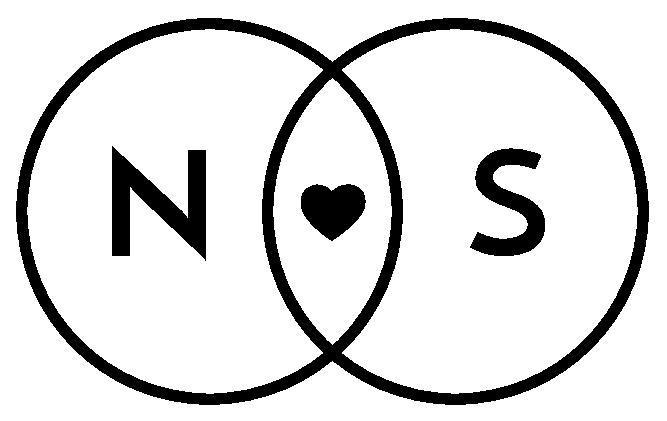
\includegraphics[scale=0.23]{img/Logo_piccolo.eps}
\vfill
\LARGE\NSposo \ e \NSposa\\
\small15 Settembre 2018\\
\end{figure}
\vfill
\Huge \textbf{Menu}\\
\hfill\break
\normalsize\textbf{Aperitivo e antipasto a buffet}\\
\hfill\break
\textbf{Primi piatti}\\
Riso Carnaroli al Franciacorta brut, frutti di mare caramellati e polvere di mandarino\\
\hfill\break
Lasagnetta aperta agli spinaci con brasatello di cervo e fonduta di Maniva DOP\\
\hfill\break
\textbf{Secondo piatto}\\
Filetto di manzo alla rosa marinato ai mirtilli rossi in crosta di erbe fini e ginepro\\
\hfill\break
\textbf{Torta nuziale}\\
\textbf{Buffet di dolci e frutta}\\
\textbf{Caffè}\\

\vfill

\begin{center}

\includegraphics[scale=0.1]{img/cuori_venn.eps}
\end{center}

\vfill

\end{center}

\noindent\scriptsize\textbf{Vini:}\\
Franciacorta Brut “Tenuta delle Farfalle” Cantine Monzio Compagnoni\\
%\footnotesize
“Ottava Rima” 2014 Maremma Doc Tenuta L’Impostino\\
Lugana 2016 Azienda Agricola Bertagna\\
Moscato d’Asti Tenuta Marcarini\\

\begin{figure}[h!]
\centering
\def\svgscale{0.5}\input{img/logo-cnb-org_black.pdf_tex}
\end{figure}

\end{document}